\documentclass[conference]{IEEEtran}
\usepackage[top=2.5 cm, bottom=2.5 cm, left=2.0 cm, right=2.0 cm]{geometry}
\geometry{letterpaper}
\usepackage[parfill]{parskip}
\usepackage{graphicx}
\usepackage{amsmath}
\usepackage{amssymb}
\usepackage{comment}
\usepackage{epstopdf}
\usepackage{subfigure}
\usepackage{extarrows}
\usepackage{minted}
\usepackage{tensor}
\usemintedstyle{vs}
\usepackage{kbordermatrix}

\DeclareGraphicsRule{.tif}{png}{.png}{`convert #1 `dirname #1`/`basename #1 .tif`.png}



\title{Realtime 6DOF SLAM for a Quadrotor Helicopter}

\author{\IEEEauthorblockN{Stephen Chaves}
  \and
  \IEEEauthorblockN{Schuyler Cohen}
  \and
  \IEEEauthorblockN{Patrick O'Keefe}
  \and
  \IEEEauthorblockN{Paul Ozog}}

% \IEEEauthorblockA{School of Electrical and\\Computer Engineering\\
% Georgia Institute of Technology\\
% Atlanta, Georgia 30332--0250\\
% Email: http://www.michaelshell.org/contact.html}



\begin{document}
\maketitle



\begin{abstract}
  Lorem ipsum dolor sit amet, consectetur adipisicing elit, sed do eiusmod tempor incididunt
  ut labore et dolore magna aliqua. Ut enim ad minim veniam, quis nostrud exercitation
  ullamco laboris nisi ut aliquip ex ea commodo consequat. Duis aute irure dolor in
  reprehenderit in voluptate velit esse cillum dolore eu fugiat nulla pariatur. Excepteur
  sint occaecat cupidatat non proident, sunt in culpa qui officia deserunt mollit anim id
  est laborum.
\end{abstract}






\section{Introduction}
\label{sec:introduction}

% Schuyler's section

Lorem ipsum dolor sit amet, consectetur adipisicing elit, sed do eiusmod tempor incididunt
ut labore et dolore magna aliqua. Ut enim ad minim veniam, quis nostrud exercitation
ullamco laboris nisi ut aliquip ex ea commodo consequat. Duis aute irure dolor in
reprehenderit in voluptate velit esse cillum dolore eu fugiat nulla pariatur. Excepteur
sint occaecat cupidatat non proident, sunt in culpa qui officia deserunt mollit anim id
est laborum.




\section{System Architecture}
\label{sec:systemarchitecture}

% Steve's Section

The architecture of our SLAM software was developed with modularity and versatility in
mind.  As a result, the SLAM software essentially consists of two sides: a front-end that
interfaces with the robot and produces a graph of nodes and edges from odometry and
landmark observations, and a back-end that solves the SLAM problem from this graph.

In our framework, each robot node is a six dimensional pose and each landmark node is a
three dimensional position. These poses and positions make up the state vector solved by
the back-end.  The edges represent relative poses between two nodes. The relative pose
between two robot nodes is an odometry edge, and the relative pose between a landmark node
and a robot node is an observation edge. These relative poses are the constraints that the
back-end SLAM solver uses to optimize the estimate of the state vector. Together, the
nodes and edges form a graph representation of the SLAM problem.  \S\ref{sec:6dof}
describes the mathematical 6-DOF spatial relationships we use frequently in our graph
representation.


For passing information between the front-end and back-end, we employ the Lightweight
Communications and Marshalling (LCM) library. \cite{huang2010} The front-end also uses LCM
to receive data from the robot and send it motion commands.

By designing the software in a modular framework, the back-end is a generic solver for any
graph-based SLAM problem. Thus, the back-end can be easily transferred between SLAM
applications. Only the front-end is specific to the application. The back-end solver we
implemented is called incremental smoothing and mapping (iSAM), and is discussed in the
following section. However, because of its modularity, other back-end SLAM solvers (like
batch methods, for example) can be inserted without alteration to the front-end.


\section{Incremental Smoothing and Mapping}
\label{sec:incrementalsmoothingandmapping}

%Pat's section

Incremental smoothing and mapping (iSAM) is a relatively recent approach to solving the
full SLAM problem. \cite{Kaess08tro} The full SLAM problem, in contrast to the online SLAM
problem, recovers the full posterior of the robot trajectory and landmark positions
instead of just the current robot pose and landmark positions. \cite{thrun2005probabilistic}

In standard least-squares SLAM, we solve a system of equations such as

\begin{align*}
  \Delta x' &= \underset{\Delta x}{\operatorname{argmin}} (J\Delta x - r)^{\text{T}}
\Sigma^{-1} (J\Delta x - r) \\
  &= \underset{\Delta x}{\operatorname{argmin}} \| J\Delta x - r \|^2_{\Sigma}
\end{align*}

where $x$ is the state vector that contains all robot poses and
landmark positions, $J$ is the Jacobian of the observation model that
predicts measurements given the state vector, $\Delta x$ is the
deviation of $x$ from the linearization point, and $r$ is the residual
of observations versus the predicted measurements. The minimizing
solution results in the standard normal equations.

\[
(J^{\text{T}} \Sigma^{-1} J) \Delta x = J^{\text{T}} \Sigma^{-1}r
\]

This is solved via the Cholesky decomposition of the information matrix,
$J^{\text{T}}\Sigma^{-1}J$.

iSAM makes a change to this problem formulation by considering the Cholesky decomposition
of $\Sigma^{-1}$ -- written as $\Sigma^{-\text{T}/2}$ to denote the upper triangular
result of the decomposition --  and rewriting the least squares problem as

\begin{align*}
    \Delta x' &= \underset{\Delta x}{\operatorname{argmin}} (J\Delta x - r)^{\text{T}}
\Sigma^{-1/2}\Sigma^{-\text{T}/2} (J\Delta x - r) \\
  &= \underset{\Delta x}{\operatorname{argmin}} \| \Sigma^{-\text{T}/2}(J\Delta x - r)
  \|^2\\
&= \underset{\Delta x}{\operatorname{argmin}} \| (A\Delta x - b)\|^2
\end{align*}

where

\begin{align*}
  A &= \Sigma^{-\text{T}/2}J \\
  b &= \Sigma^{-\text{T}/2}r
\end{align*}

This allows us to solve $A\Delta x = b$ by applying QR factorization directly to $A$. This
is advantageous because it avoids the squaring of the matrix condition number that is
associated with the normal equation form. Moreover, there is the nice property that the
$R$ that results from the QR decomposition of $A$ is equivalent to the upper triangular
term in the Cholesky decomposition of $A^{\text{T}}A$ if A is real. \cite{Kaess08tro}

iSAM recovers the posterior by doing fast incremental updates to the factorization of $A$.
This means that calculations are only performed on elements that are actually affected* by
 new measurements. We can get away with this because we often have a very good estimate of
 the state vector so doing a full batch re-linearization and solution at each step wastes
 calculations because most elements of $\Delta x$ will be zero. However, iSAM periodically
 does perform a full batch solution in order to compensate for accumulated linearization
 errors. Over time, loop closures greatly decrease the sparsity of the matrix
 factorization, so variable reordering is performed during each batch solution step. The
 incremental update and variable reordering will be covered below.


\subsection{Givens Rotations}
\label{sub:givensrotations}

The $R$ term that results from the QR decomposition of $A$ is upper triangular by
definition. When a new measurement row is added to $A$, we can incrementally update $R$
instead of performing the entire QR decomposition again. The way to achieve this is via
Givens rotations. 

Givens rotations are a way to introduce a zero at a specified point in a matrix by
premultiplying by a matrix of the form


\[
G(i, k, \theta) =
\kbordermatrix{  & & &i& &k & & \\
 & 1   & \cdots &    0   & \cdots &    0   & \cdots &    0   \\
 & \vdots & \ddots & \vdots &        & \vdots &        & \vdots \\
i & 0   & \cdots &    c   & \cdots &    -s   & \cdots &    0   \\
 & \vdots &        & \vdots & \ddots & \vdots &        & \vdots \\
k & 0   & \cdots &   s   & \cdots &    c   & \cdots &    0   \\
 & \vdots &        & \vdots &        & \vdots & \ddots & \vdots \\
 & 0   & \cdots &    0   & \cdots &    0   & \cdots &    1
       }
\] 

where $c = \cos{(\theta)}$ and $s = \sin{(\theta)}$ for some $\theta$. We follow the
  algorithms in Golub and Van Loan's \emph{Matrix Computations} to find $c$ and $s$ to
  zero a particular element in a matrix. \cite{golub1996matrix} 

When we receive new rows for $A$ when a new measurement occurs, they are appended to $R$,
which is then no longer upper-triangular. A series of Givens rotations are applied to the
elements that are below the diagonal. This is called triangularization and once the
below-diagonal elements have been removed via the rotations, the resulting
upper-triangular matrix is equivalent to the QR decomposition of the full $A$ matrix.
\cite{golub1996matrix} The same series of rotations needs to be applied to our right hand
side $b$ term.

After the rotations have been performed, the system can be solved with simple back-substitution.


\subsection{Variable Reordering}
\label{sub:variablereordering}

When a robot closes a loop, a correlation is introduced between the current pose and a
previously observed landmark. This landmark is connected to earlier poses in the
trajectory as well. These correlations greatly increase the number of non-zero elements in
the matrix factorization which in turn increases the computational complexity of updating
and solving the system. Figure \ref{fig:images/reorder32} shows the large swaths of
non-zero elements that are introduced during loop closures. 

In order to avoid this problem, we can perform variable reordering. This is essentially a
permutation of the columns of $A$ where columns that belong to the same node in the SLAM
graph are kept together. This new order influences the variable elimination which
has a profound effect on the sparsity of the factorization. Figure
\ref{fig:images/reorder33} shows the result of applying variable reordering to simulated
data that has experienced several loop closures.


\begin{figure}[!h]
  \begin{center}
    \subfigure[] {
    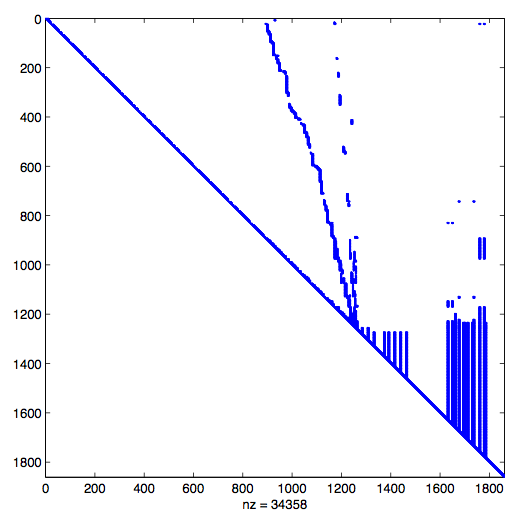
\includegraphics[width=2.5in]{images/reorder32}
    \label{fig:images/reorder32}}
    \subfigure[] {
    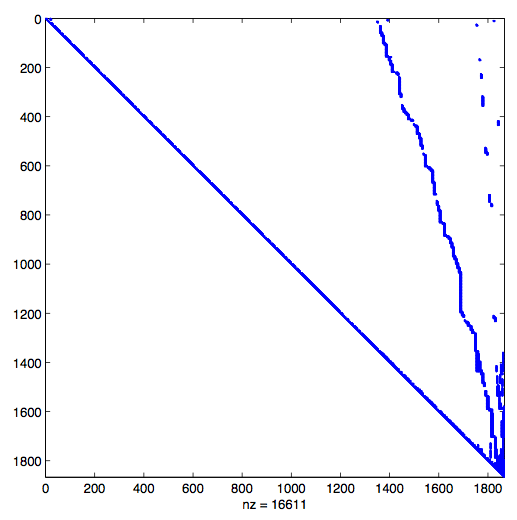
\includegraphics[width=2.5in]{images/reorder33}
    \label{fig:images/reorder33}}
    \caption{The factorization of the $A$ matrix after 300 time steps of simulated data
      that includes loop closures. (a) Before variable reordering, the loop closures
      introduce many non-zero elements. (b) After variable reordering, we have a much more
    sparse factorization. Over 50\% of the non-zero elements were removed.}
    \label{fig:reorder}
  \end{center}
\end{figure}


The best column variable ordering is NP hard, and iSAM uses COLAMD as a heuristic to
assist in the process. \cite{davis2004column} Our implementation uses a simplified
heuristic that counts the number of connected nodes in the graph. It is not the minimum
degree ordering, but we have found it to be more than adequate in our tests. Figure
\ref{fig:reorder} is an example of the application of our simplified heuristic.

\section{Back-end Motion and Observation Models}
\label{sec:backendModels}

\subsection{6-DOF Spatial Relationships}
\label{sec:6dof}
% Paul's section

We adopt the notation from~\cite{rsmith-1990a,reustice-phdthesis} to
describe three particular spatial relationships of 6-DOF coordinate
frames: {\it compound, inverse}, and {\it composite}.  This notation
allows us to abstract away the linear algebra operations necessary for
applying these relationships to nonlinear motion and observation models.

Let ${\bf x}_{ij} = \begin{bmatrix}
  {\bf t}_{ij}^i & {\boldsymbol \Theta}_{ij}\\
\end{bmatrix}^\top$ be a vector in $\mathbb{R}^6$ describing the
relative pose of frame $j$ with respect to frame $i$.  ${\bf
  t}_{ij}^i$ is the $3\times 1$ translation vector from frame $i$ to
frame $j$ as expressed in frame $i$.  ${\boldsymbol \Theta}_{ij}$ is
the $3 \times 1$ vector describing the Euler angles of the $x$, $y$,
and $z$ axes.  We define the function $(\text{rotxyz}: \mathbb{R}^3
\rightarrow \mathbb{R}^{3\times3})$ that maps a vector of Euler angles to
a rotation matrix as follows:
\begin{eqnarray*}
  R_j^i & = & \text{rotxyz}({\boldsymbol \Theta}_{ij})
\end{eqnarray*}
where $R_j^i$ is the matrix that rotates frame $j$ into frame $i$.

These definitions allow us to describe the transformation matrix
that uniquely relates homogeneous 3D points in frame $j$ to homogeneous
points in frame $i$ as:
\begin{eqnarray*}
  H_{j}^i & = & \begin{bmatrix}
    R_j^i & {\bf t}_{ij}^i\\
    {\bf 0} & 1
  \end{bmatrix}
\end{eqnarray*}
Note that given $H_j^i$, we can easily compute ${\bf x}_{ij}$ and vice
versa using April's \texttt{LinAlg} Java package.

\subsubsection{Compounding Operation}
\label{sub:compoundingoperation}

Let the $\oplus$ operator describe the spatial relationship between
two frames arranged ``head-to-tail'':
\begin{eqnarray*}
  {\bf x}_{ik} & = & {\bf x}_{ij} \oplus {\bf x}_{jk} 
\end{eqnarray*}
${\bf x}_{ik}$ can be computed from recovering the $6 \times 1$ vector
corresponding to the matrix
\begin{eqnarray*}
  H_k^i & = & H_j^i H_k^j
\end{eqnarray*}

% For example, for the compounding operation, our SLAM backend takes $i$
% to denote the world frame.  $j$ and $k$ denote the frame of the robot
% at the previous and current timesteps, respectively.  This effectively
% acts as a motion model that predicts the global pose of a robot in
% 6-DOF given the odometry at every timestep.

The Jacobian of the compounding operation $J_\oplus$ is given
in~\cite{reustice-phdthesis}.  Using this matrix, we can compute to
first order the covariance of ${\bf x}_{ik}$ as
\begin{eqnarray*}
  \Sigma({\bf x}_{ij}) & = & J_\oplus \begin{bmatrix}
    \Sigma({\bf x}_{ik}) & \Sigma({\bf x}_{ij}, {\bf x}_{kj})\\
    \Sigma({\bf x}_{kj}, {\bf x}_{ij}) & \Sigma({\bf x}_{kj})\\
  \end{bmatrix} J_\oplus^\top
\end{eqnarray*}

\subsubsection{Inverse Operation}
\label{sub:inverseoperation}
Let the $\ominus$ operator describe the inverse of a relative pose
vector:
\begin{eqnarray*}
  {\bf x}_{ji} & = & \ominus {\bf x}_{ij}
\end{eqnarray*}
This operation is computed from the transformation matrix
\begin{eqnarray*}
  H_i^j & = & \left(H_j^i\right)^{-1} \\
  & = & \begin{bmatrix}
    \left( R_j^i \right)^\top & -\left( R_j^i \right)^\top {\bf t}_{ij}^i\\
    {\bf 0} & 1
  \end{bmatrix}
\end{eqnarray*}
The first-order covariance projection of this operation is
\begin{eqnarray*}
  \Sigma({\bf x}_{ji}) & = & J_\ominus \Sigma({\bf x}_{ij}) J_\ominus^\top
\end{eqnarray*}
where the closed-form expression for the Jacobian is given
in~\cite{reustice-phdthesis}.

\subsubsection{Composition Operation}
\label{sub:compositionoperation}
We define the composite operation on two frames related
``tail-to-tail'' using the compounding and inverse operations:
\begin{eqnarray*}
  {\bf x}_{jk} & = & \ominus {\bf x}_{ij} \oplus {\bf x}_{ik}
\end{eqnarray*}
where the Jacobian of this relationship is 
\begin{eqnarray*}
  \tensor[_\ominus]{J}{_\oplus} & = & J_\oplus \begin{bmatrix}
    J_\ominus & 0_{6 \times 6}\\
    0_{6 \times 6} & I_{6 \times 6}\\
  \end{bmatrix}
\end{eqnarray*}
and thus the first-order covariance projection of the composite
operation is
\begin{eqnarray*}
  \Sigma({\bf x}_{jk}) & = & \tensor[_\ominus]{J}{_\oplus} \begin{bmatrix}
    \Sigma({\bf x}_{ij}) & \Sigma({\bf x}_{ij}, {\bf x}_{ik})\\
    \Sigma({\bf x}_{ik}, {\bf x}_{ij}) & \Sigma({\bf x}_{ik})\\
  \end{bmatrix} \tensor[_\ominus]{J}{_\oplus^\top}
\end{eqnarray*}
% An example application of this composite operation is to estimate the
% odometry of a robot between two successive timesteps (given the
% current and previous poses of the robot in the global frame).  In this
% case, $i$ is the global frame, $j$ is the frame of the robot at the
% previous timestep, and $k$ is the robot frame at the current timestep.
% ${\bf x}_{jk}$ is then the predicted odometry between frame $j$ and
% frame $k$.



\subsection{Node Initialization}
\label{sub:nodeinitializationandedgeresiduals}
Every timestep in which the robot moves or a feature is observed, a new node is created
and initialized.  To initialize a node means to assign that node a pose (for robot poses)
or a point (for landmarks) in the global frame.  This is computed by the measurement
that relates the new node to a previous node.  To initialize a node without connecting to
a previously created node is a referred to as adding a ``prior.''

For the following sections, let $g$ represent the global frame.  For each node, a
first-order covariance projection can be computed as in Section~\ref{sec:6dof}.

\subsubsection{Pose Nodes}
\label{subs:posenodeinit}

Say frame $i$ corresponds to an initialized pose node in the SLAM graph.  We observe a
odometry measurement relating frame $i$ and frame $j$.  Then we initialize node $j$ to be
in the global frame with the ``head-to-tail'' operation $ {\hat {\bf x}_{gj}} = {\bf
  x}_{gi} \oplus {\bf x}_{ij} $

\subsubsection{Landmark Nodes}
\label{subs:pointnodeinit}
Given the relative {\it position} of a landmark frame $l$ with respect to robot frame $i$,
we construct a relative {\it pose} vector by setting the orientation of $l$ to be
arbitrary.  Then, the relative {\it position} of the landmark in the global frame is the
translation vector corresponding to $ {\hat {\bf x}}_{gl} = {\bf x}_{gi} \oplus {\bf
 x}_{il} $

\subsection{Factor Computation}
\label{sub:nodeinitializationandedgeresiduals}

To solve the least squares problem described in
\S\ref{sec:incrementalsmoothingandmapping}, we need to compute a observation model
Jacobian $J$ and residual vector $r$.  Together, these comprise a ``factor'' between two
unknowns in the graph.  In the following section, we describe how these are computed using
the notation from \S\ref{sec:6dof}.

\subsubsection{Pose-to-Pose Factors}
\label{subs:posenodelinear}
Given two guesses of robot frames $i$ and $j$ (with respect to the global frame), then the
predicted relative pose observation is $ {\hat {\bf x}_{ij}} = \ominus {\bf x}_{gi} \oplus
{\bf x}_{gj}$. The Jacobian of this relationship is evaluated as in
\S\ref{sub:compositionoperation}.  The residual vector is simply the difference
between the predicted ${\hat {\bf x}_{ij}}$ and the observed ${\bf x}_{ij}$.

\subsubsection{Pose-to-Landmark Factors}
\label{subs:pointnodelinear}

If a landmark $l$ is observed frame robot frame $i$, then we can predict this measurement
by the ``tail-to-tail'' operation.  We simply assign the orientation of ${\bf x}_{gl}$ to
be arbitrary.  Then, the estimated observation is the translational component of $ {\hat
  {\bf x}}_{il} = \ominus {\bf x}_{gi} \oplus {\bf x}_{gl} $. The residual for the
landmark is the difference between this prediction and what the robot actually measured.

Note that for the computation of this factor's Jacobian, we drop the differentiations with
respect to the orientation of the landmark.  This leaves us with a $3 \times 9$ Jacobian
and $3 \times 3$ positional covariance matrix.

\section{AprilTag Relative Pose Covariance Estimate}
\label{sec:apriltags}

% Paul's section

We used the AprilTag system throughout our project's experiments and demonstrations for
relative position and orientation.  The accuracy, detection performance, and small memory
footprint made it particularly desirable~\cite{olson2011tags}.

We applied principles of linearized covariance projection to estimate a covariance matrix
for the 6-DOF relative pose vector ${\bf x}_{tc}$ that describes the relative pose from
the tag's frame $t$ to the camera's frame $c$.

Denote $f$ as the function that computes the $9 \times 1$ homography vector ${\bf h}$ from
a set of world points and image points via the Direct Linear Transform (DLT) algorithm.
By linearizing $f$ around a mean input (the observed image point coordinates), we can
compute the $9 \times 9$ covariance matrix $\Sigma({\bf h})$ to first order.  From there,
we project the covariance estimate of $h$ by linearizing a function $g$, which maps the
homography to ${\bf x}_{tc}$.

For simplicity, we assume that the uncertainty of the world points and the camera
calibration parameters are zero.  Further, we assume negligible lens distortion.  All
differentiations are done numerically.

Under these assumptions, the covariance estimate of the relative pose from tag to camera
is simply
\begin{eqnarray*}
  \Sigma({{\bf x}_{tc}}) & = & J_g J_f \Sigma({\bf u}) J_f^\top J_g^\top
\end{eqnarray*}
where ${\bf u}$ is the $2N \times 1$ vector of $N$ noisy image point coordinates and
$\Sigma({\bf u})$ is the associated isotropic covariance matrix.  We assume the feature
noises are independent. The diagonal elements of this covariance matrix are tuned by the
user.

The Jacobians are computed by finite difference:
\begin{align*}
  \left[J_f\right]_{ij} &=\frac{\partial f_i}{\partial u_j} \\
  &= \frac{f_i(u_0, u_1, \dots, u_i +
    \epsilon, \dots, u_{2N})}{\epsilon} \\
  & \ \ \  - \frac{f_i(u_0, \dots, u_{2N})}{\epsilon}
\end{align*}
for some small $\epsilon$. One should note that when differentiating $f$, the homography
vectors must have the same sign.  This is not guaranteed in typical Singular Value
Decomposition (SVD) libraries because the sign of the singular vectors may be flipped when
the input matrix is slightly perturbed.

Also, we take $g$ to directly map the homography to ${\bf x}_{tc}$.  The covariance
projections operations referred to in \S\ref{sec:6dof} are therefore included in $g$.

%Just to see how it looks using both columns
\begin{figure*}[!t]
  \begin{center}
    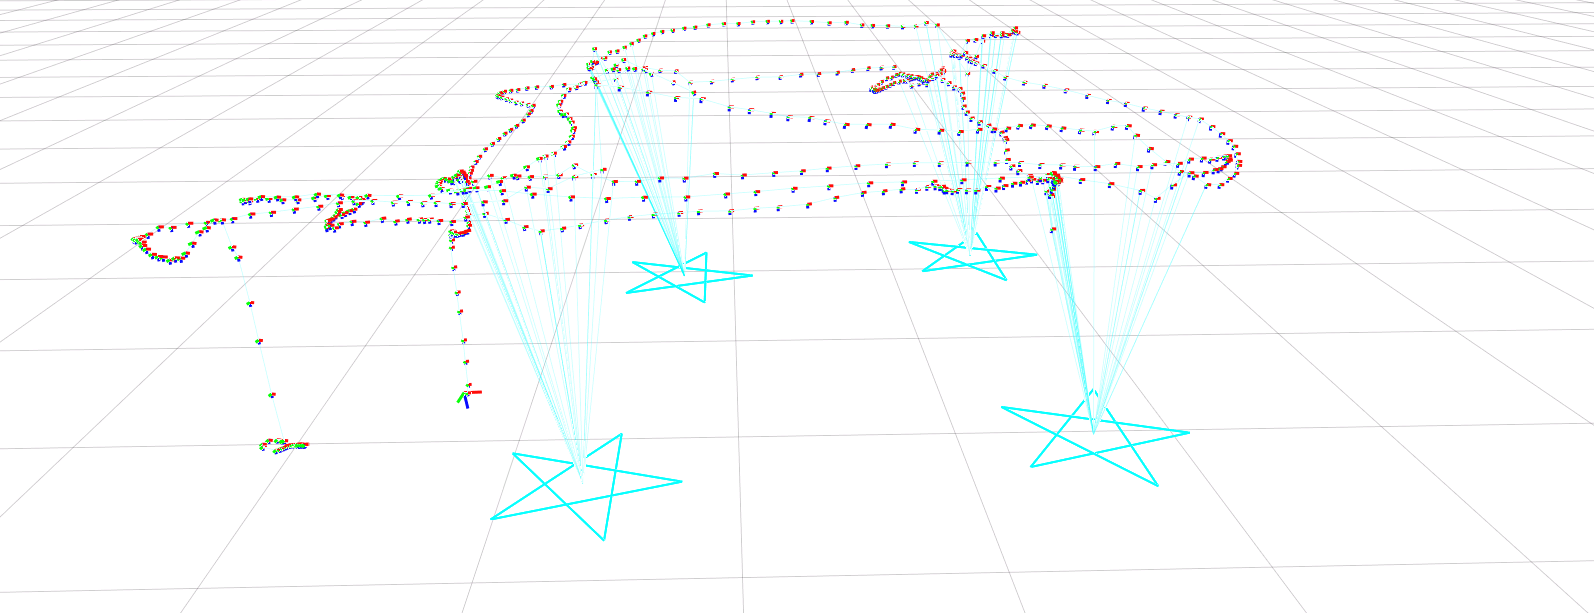
\includegraphics[width=1.0\textwidth]{images/square}
    \caption{asdf}
    \label{fig:square}
  \end{center}
\end{figure*}



\section{Experiments}
\label{sec:experiments}

Lorem ipsum dolor sit amet, consectetur adipisicing elit, sed do eiusmod tempor incididunt
ut labore et dolore magna aliqua. Ut enim ad minim veniam, quis nostrud exercitation
ullamco laboris nisi ut aliquip ex ea commodo consequat. Duis aute irure dolor in
reprehenderit in voluptate velit esse cillum dolore eu fugiat nulla pariatur. Excepteur
sint occaecat cupidatat non proident, sunt in culpa qui officia deserunt mollit anim id
est laborum.


\subsection{Simulation}
\label{sub:simulation}

% Pat's section

Lorem ipsum dolor sit amet, consectetur adipisicing elit, sed do eiusmod tempor incididunt
ut labore et dolore magna aliqua. Ut enim ad minim veniam, quis nostrud exercitation
ullamco laboris nisi ut aliquip ex ea commodo consequat. Duis aute irure dolor in
reprehenderit in voluptate velit esse cillum dolore eu fugiat nulla pariatur. Excepteur
sint occaecat cupidatat non proident, sunt in culpa qui officia deserunt mollit anim id
est laborum.

\begin{figure}[!t]
  \centering
  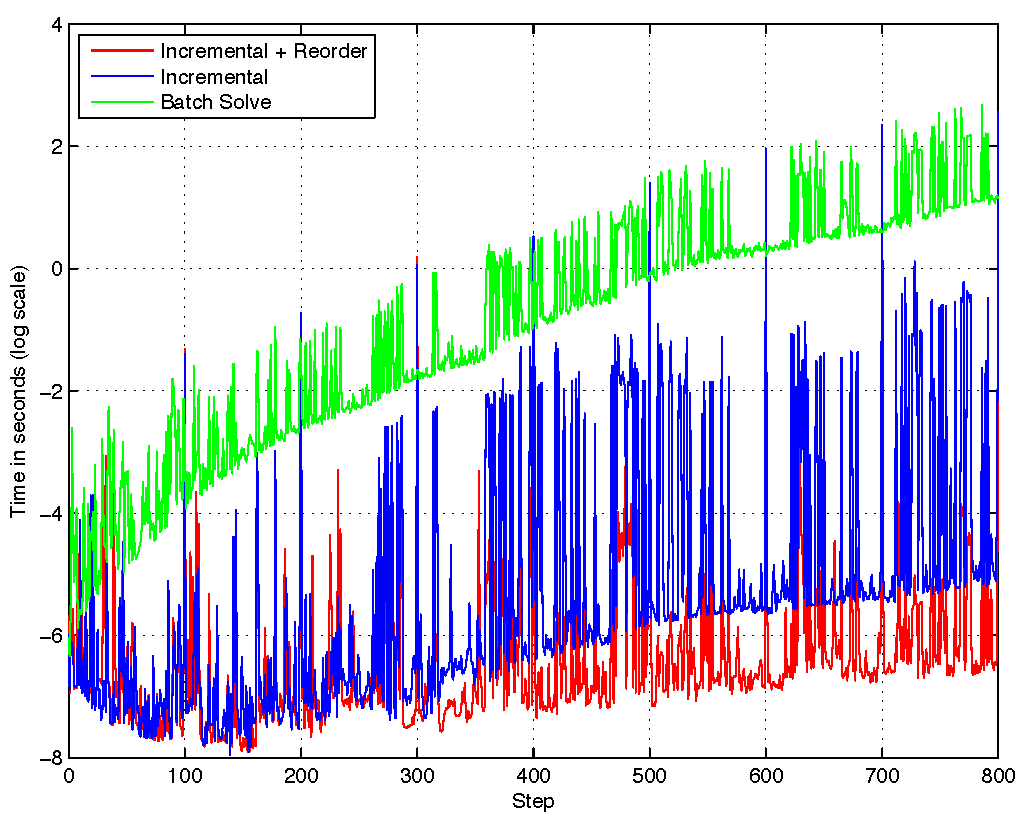
\includegraphics[width=2.5in]{images/stepTimeResults}
  \caption{The time per step for different SLAM solve methods.}
  \label{fig:stepTime}
\end{figure}

\subsection{Parrot AR.Drone}
\label{sub:quadrotor}

% Steve talks about drone hardware
% Schuyler gets results

The quadrotor helicopter we used for experimental testing of the realtime 6-DOF SLAM algorithm
was a Parrot AR.Drone. Despite its reputation as an augmented reality gaming platform (for which
it is markteted), the AR.Drone has a substantial robotics community. The AR.Drone has a full 
suite of MEMS inertial sensors: a three-axis accelerometer, a two-axis gyroscope for measuring 
pitch and roll, and a yaw angle precision gyroscope.  It also features an ultrasound altimeter
and two cameras for recording images in the forward-looking and downward-looking directions.

\begin{figure}[!h]
  \centering
  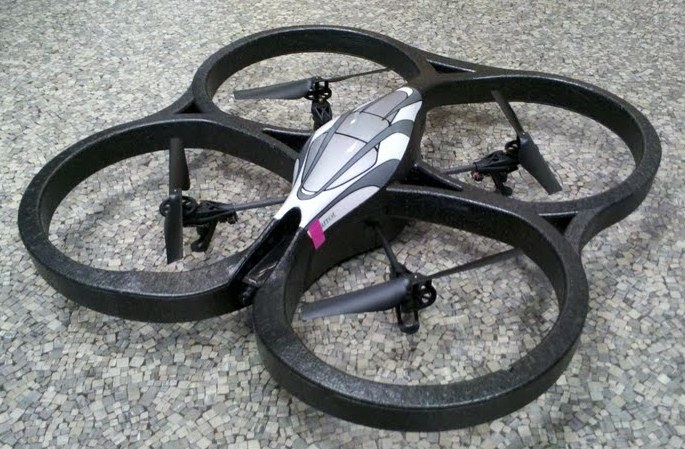
\includegraphics[width=2.5in]{images/drone1}
  \caption{The Parrot AR.Drone used for experimental testing.}
  \label{fig:drone}
\end{figure}

The downward-looking camera was used to detect AprilTags acting as landmarks in our environment.
The AR.Drone itself fuses measurements from its inertial sensors and cameras to provide estimates 
of the velocities and Euler angles along its principal axes. The front-end we implemented manipulates these
measurements, along with the AR.Drone's reported altitude, into relative poses (quadrotor odometry).
Both the camera images and state measurements are transmitted by the AR.Drone over its own
wireless ad-hoc network and read into the front-end using LCM.


Lorem ipsum dolor sit amet, consectetur adipisicing elit, sed do eiusmod tempor incididunt
ut labore et dolore magna aliqua. Ut enim ad minim veniam, quis nostrud exercitation
ullamco laboris nisi ut aliquip ex ea commodo consequat. Duis aute irure dolor in
reprehenderit in voluptate velit esse cillum dolore eu fugiat nulla pariatur. Excepteur
sint occaecat cupidatat non proident, sunt in culpa qui officia deserunt mollit anim id
est laborum.

\subsection{Interactive Demonstration}
\label{sub:interactiveDemo}

\begin{figure}[!h]
  \begin{center}
    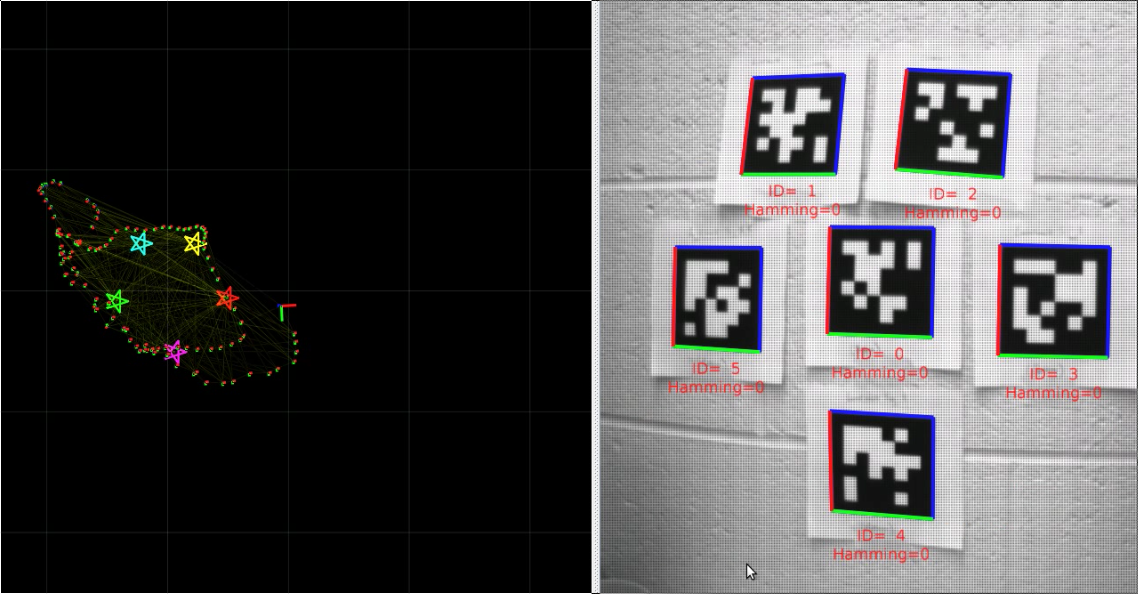
\includegraphics[width=2.5in]{images/interactiveDemo}
    \caption{asdf}
    \label{fig:interactiveDemo}
  \end{center}
\end{figure}


\section{Conclusion}
\label{sec:conclusion}

% Schuyler's section

Lorem ipsum dolor sit amet, consectetur adipisicing elit, sed do eiusmod tempor incididunt
ut labore et dolore magna aliqua. Ut enim ad minim veniam, quis nostrud exercitation
ullamco laboris nisi ut aliquip ex ea commodo consequat. Duis aute irure dolor in
reprehenderit in voluptate velit esse cillum dolore eu fugiat nulla pariatur. Excepteur
sint occaecat cupidatat non proident, sunt in culpa qui officia deserunt mollit anim id
est laborum.



\section{Acknowledgment}

The authors would like to thank Sprite, the number 7, and Emacs.



\bibliographystyle{IEEEtran}
% argument is your BibTeX string definitions and bibliography database(s)
\bibliography{IEEEabrv,references}


\end{document}



% An example of a floating table. Note that, for IEEE style tables, the
% \caption command should come BEFORE the table. Table text will default to
% \footnotesize as IEEE normally uses this smaller font for tables.
% The \label must come after \caption as always.
%
% \begin{table}[!t]
%%   increase table row spacing, adjust to taste
%   \renewcommand{\arraystretch}{1.3}
%   if using array.sty, it might be a good idea to tweak the value of
%   \extrarowheight as needed to properly center the text within the cells
%   \caption{An Example of a Table}
%   \label{table_example}
%   \centering
%%   Some packages, such as MDW tools, offer better commands for making tables
%%   than the plain LaTeX2e tabular which is used here.
%   \begin{tabular}{|c||c|}
%     \hline
%     One & Two\\
%     \hline
%     Three & Four\\
%     \hline
%   \end{tabular}
% \end{table}
